\documentclass[11pt,a4paper]{article}

\usepackage[T1]{fontenc}
\usepackage{lmodern}
\usepackage[margin=2.4cm]{geometry}
\usepackage{amsmath,amssymb,amsthm}
\usepackage{booktabs}
\usepackage{siunitx}
\usepackage{microtype}
\usepackage{pgfplots}
\pgfplotsset{compat=1.16}
\usepackage[colorlinks=true,linkcolor=blue!50!black,citecolor=blue!50!black,urlcolor=blue!50!black]{hyperref}
\usepackage[capitalise,noabbrev]{cleveref}
\usepackage{authblk}
\usepackage[skip=6pt,font=small,labelfont=bf]{caption}

\newtheorem{proposition}{Proposition}
\newtheorem{corollary}[proposition]{Corollary}
\theoremstyle{definition}
\newtheorem{definition}{Definition}
\theoremstyle{remark}
\newtheorem{remark}{Remark}

\newcommand{\dd}{\mathrm{d}}
\newcommand{\mrel}{m_{\mathrm{rel}}}
\newcommand{\dimof}[1]{\left[\,#1\,\right]}
\newcommand{\sfM}{\mathsf{M}}
\newcommand{\sfL}{\mathsf{L}}
\newcommand{\sfT}{\mathsf{T}}

\title{\textbf{On the Apparent $\infty\cdot 0$ Indeterminacy of\\
Relativistic Mass and Length Contraction:\\
A Dimensional and Covariant Analysis of the $v\to c$ Boundary}}

\author{Author Name}
\affil{Affiliation}
\date{November 2026}

\begin{document}
\maketitle

\begin{abstract}
\noindent
Heuristic arguments in special relativity often combine the growth of
``relativistic mass'' $\mrel=\gamma m$ with the Lorentz contraction
$L=L_0/\gamma$ and conclude that the limit $v\to c$ produces an
indeterminate form of type $\infty\cdot 0$, or that it equates a divergent
mass--time product with a divergent length. We examine the schematic boundary
statement
$X=\lim_{v\to c}(\infty\,M\cdot T)=\infty\,(xL)$
and show that (i) it admits no dimensionally consistent left-hand side $X$ in
SI, natural ($\hbar=c=1$), or geometrized ($G=c=1$) units; (ii) the only
monomial in $G$, $c$, $\hbar$ that could restore consistency is
$\kappa=\sqrt{Gc/\hbar}=c/m_P$; and (iii) the alleged indeterminacy is absent,
since $\mrel L\equiv mL_0$ identically for all $v<c$. A covariant treatment
based on the stress--energy tensor of pressureless dust confirms which
quantities diverge (energy, momentum, mass per unit length, dilated time) and
which remain finite and Lorentz-invariant. A $\gamma$-power-counting rule
classifies all such products. We close by giving a well-posed boundary
relation with genuine dimension of length that diverges in the limit, the
laboratory distance covered in a fixed proper time,
$\Delta x=p\tau_0/m=c\tau_0\sinh\eta$.
\end{abstract}

\section{Introduction}\label{sec:intro}

The Lorentz factor
\begin{equation}
  \gamma(v)=\left(1-\frac{v^2}{c^2}\right)^{-1/2}, \qquad 0\le v<c,
  \label{eq:gamma}
\end{equation}
diverges as $v\to c^-$. Several textbook kinematic effects scale as positive
or negative powers of $\gamma$: the energy $E=\gamma mc^2$, the contracted
length $L=L_0/\gamma$ of a rod measured along its direction of motion, and the
dilated coordinate time $\Delta t=\gamma\tau_0$ corresponding to a proper
interval $\tau_0$~\cite{Einstein1905,TaylorWheeler,Rindler}. Products of such
quantities are sometimes presented as paradoxical: one factor grows without
bound while another vanishes, and the product is then described as an
indeterminate form whose value at the light-speed ``boundary'' is assumed to
be something non-trivial.

In this note we analyse a representative statement of this kind,
\begin{equation}
  X \;=\; \lim_{v\to c}\bigl(\infty\,M\cdot T\bigr) \;=\; \infty\,(xL),
  \label{eq:claim}
\end{equation}
where $M$ is a mass, $T$ a time, $L$ a length and $x$ a dimensionless number.
We ask three questions: what physical quantity $X$ could stand on the left;
whether the product of relativistic mass and contracted length is genuinely
indeterminate; and what covariant statement survives once the heuristics are
removed. Throughout, $m$ denotes the invariant (rest) mass. We use the term
``relativistic mass'' $\mrel\equiv E/c^2=\gamma m$ only to engage with the
heuristic. Its use is discouraged in modern
treatments~\cite{Okun1989,TaylorWheeler}.

\section{Dimensional analysis}\label{sec:dims}

Writing $\dimof{\cdot}$ for the dimension of a quantity in the base
$\{\sfM,\sfL,\sfT\}$~\cite{Bridgman}, the two sides of \cref{eq:claim} carry
\begin{equation}
  \dimof{M\,T}=\sfM\sfT,\qquad \dimof{x\,L}=\sfL.
  \label{eq:dims}
\end{equation}
The symbol $\infty$ denotes a limiting process and carries no dimension.
Consistency would require $\sfM\sfT=\sfL$. \Cref{tab:units} shows that this
fails in all common systems of units.

\begin{table}[h]
  \centering
  \caption{Dimension of $M\cdot T$ under common unit conventions. In no case
  does it reduce to $\sfL$.}
  \label{tab:units}
  \begin{tabular}{@{}lcccc@{}}
    \toprule
    Convention & $\dimof{M}$ & $\dimof{T}$ & $\dimof{MT}$ & $=\sfL$? \\
    \midrule
    SI                         & $\sfM$       & $\sfT$ & $\sfM\sfT$ & no \\
    $c=1$                      & $\sfM$       & $\sfL$ & $\sfM\sfL$ & no \\
    $\hbar=c=1$ (natural)      & $\sfL^{-1}$  & $\sfL$ & $1$        & no \\
    $G=c=1$ (geometrized)      & $\sfL$       & $\sfL$ & $\sfL^{2}$ & no \\
    \bottomrule
  \end{tabular}
\end{table}

\begin{proposition}[No admissible left-hand side]\label{prop:noX}
There is no physical quantity $X$ such that $\dimof{X}=\dimof{MT}$ and
$\dimof{X}=\dimof{xL}$ simultaneously in any of the conventions of
\cref{tab:units}. Hence \cref{eq:claim}, read literally, is not a valid
physical equation.
\end{proposition}

\begin{proof}
Immediate from \cref{eq:dims} and \cref{tab:units}: in each row
$\dimof{MT}\neq\sfL$.
\end{proof}

Consistency can be restored only by multiplying the left-hand side by a
constant $\kappa$ with $\dimof{\kappa}=\sfL\,\sfM^{-1}\sfT^{-1}$.

\begin{proposition}[Unique fundamental rescaling]\label{prop:kappa}
Among monomials $G^{a}c^{b}\hbar^{d}$, the unique one with dimension
$\sfL\,\sfM^{-1}\sfT^{-1}$ is
\begin{equation}
  \kappa=\sqrt{\frac{Gc}{\hbar}}=\frac{c}{m_P}
  \approx \SI{1.378e16}{\metre\per\kilogram\per\second},
  \qquad m_P\equiv\sqrt{\frac{\hbar c}{G}} .
  \label{eq:kappa}
\end{equation}
\end{proposition}

\begin{proof}
With $\dimof{G}=\sfL^3\sfM^{-1}\sfT^{-2}$, $\dimof{c}=\sfL\sfT^{-1}$ and
$\dimof{\hbar}=\sfM\sfL^2\sfT^{-1}$, matching exponents gives the linear system
$3a+b+2d=1$, $-a+d=-1$, $-2a-b-d=-1$. Its unique solution is
$a=b=\tfrac12$, $d=-\tfrac12$.
\end{proof}

The rescaled product $\kappa MT=(M/m_P)\,cT$ is a light-travel distance
weighted by mass in Planck units. It is dimensionally sound, but it is a
construction, not an established physical law. It is recorded here only to
show what \cref{eq:claim} would minimally require.

\section{The product of relativistic mass and contracted length}\label{sec:product}

Let a rod of rest mass $m$ and rest length $L_0$ move with speed $v$ along its
length. In the laboratory frame,
\begin{equation}
  \mrel(v)=\gamma(v)\,m\xrightarrow[v\to c^-]{}\infty,
  \qquad
  L(v)=\frac{L_0}{\gamma(v)}\xrightarrow[v\to c^-]{}0 .
  \label{eq:factors}
\end{equation}

\begin{proposition}[No indeterminacy]\label{prop:product}
For every $0\le v<c$,
\begin{equation}
  \mrel(v)\,L(v)=mL_0,
  \qquad\text{hence}\qquad
  \lim_{v\to c^-}\mrel L=mL_0 .
  \label{eq:product}
\end{equation}
\end{proposition}

\begin{proof}
$\mrel L=(\gamma m)(L_0/\gamma)=mL_0$ pointwise on $[0,c)$, because
$\gamma\ge1>0$. A constant function has that constant as its limit.
\end{proof}

\begin{remark}
The phrase ``indeterminate form $\infty\cdot0$'' describes the limits of the
individual factors. It says nothing about their product, which must be found
from the functions themselves. Here the product is constant before the limit
is taken, so the indeterminacy is only apparent. Since $m$ and $L_0$ are both
frame-independent, $mL_0$ is a Lorentz scalar.
\end{remark}

\subsection{Which time?}\label{sec:time}

The symbol $T$ in \cref{eq:claim} is ambiguous, and the two readings give
opposite results:
\begin{align}
  \text{proper time, } \Delta\tau=\Delta t/\gamma:&\qquad
  \mrel\,\Delta\tau=m\,\Delta t \quad(\text{finite for fixed }\Delta t),
  \label{eq:proper}\\
  \text{dilated time, } \Delta t=\gamma\tau_0:&\qquad
  \mrel\,\Delta t=\gamma^{2}m\tau_0\xrightarrow[v\to c^-]{}\infty .
  \label{eq:dilated}
\end{align}
Only the second reading produces a divergence, and its dimension is
$\sfM\sfT$, not $\sfL$, in agreement with \cref{prop:noX}.

\subsection{A power-counting rule}\label{sec:power}

Each kinematic quantity considered here behaves as $Q\propto\gamma^{n_Q}$ at
fixed rest-frame data (note that $\gamma\beta\to\gamma$ as $\beta\to1$). A product
$Q_1Q_2\propto\gamma^{n_1+n_2}$ therefore diverges, stays finite, or vanishes
according to whether $n_1+n_2$ is positive, zero, or negative. \Cref{tab:power}
lists the exponents.

\begin{table}[h]
  \centering
  \caption{Leading $\gamma$-exponents of laboratory-frame quantities at fixed
  rest-frame data ($\beta=v/c$).}
  \label{tab:power}
  \begin{tabular}{@{}llc@{}}
    \toprule
    Quantity & Expression & $n_Q$ \\
    \midrule
    Energy / relativistic mass  & $E=\gamma mc^2$, $\ \mrel=\gamma m$ & $+1$ \\
    Momentum                    & $p=\gamma m v$                      & $+1$ \\
    Dilated time                & $\Delta t=\gamma\tau_0$             & $+1$ \\
    Number density              & $n=\gamma n_0$                      & $+1$ \\
    Mass per unit length        & $\lambda=\gamma^{2}m/L_0$           & $+2$ \\
    Contracted length           & $L=L_0/\gamma$                      & $-1$ \\
    Proper time (fixed $\Delta t$) & $\Delta\tau=\Delta t/\gamma$     & $-1$ \\
    \bottomrule
  \end{tabular}
\end{table}

\begin{figure}[h]
  \centering
  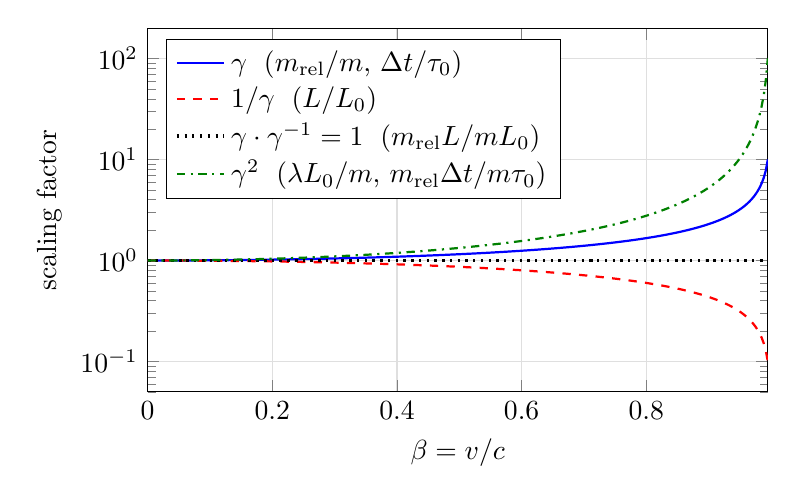
\begin{tikzpicture}
    \begin{semilogyaxis}[
      width=0.78\linewidth, height=6.2cm,
      xlabel={$\beta=v/c$}, ylabel={scaling factor},
      xmin=0, xmax=0.995, ymin=0.05, ymax=200,
      legend pos=north west, legend cell align=left,
      grid=major, grid style={gray!25},
      samples=300, domain=0:0.995,
      every axis plot/.append style={thick}]
      \addplot[blue]           {1/sqrt(1-x^2)};
      \addlegendentry{$\gamma$ \;($\mrel/m$, $\Delta t/\tau_0$)}
      \addplot[red, dashed]    {sqrt(1-x^2)};
      \addlegendentry{$1/\gamma$ \;($L/L_0$)}
      \addplot[black, dotted, very thick] {1};
      \addlegendentry{$\gamma\cdot\gamma^{-1}=1$ \;($\mrel L/mL_0$)}
      \addplot[green!50!black, dashdotted] {1/(1-x^2)};
      \addlegendentry{$\gamma^{2}$ \;($\lambda L_0/m$, $\mrel\Delta t/m\tau_0$)}
    \end{semilogyaxis}
  \end{tikzpicture}
  \caption{Scaling of laboratory-frame quantities with $\beta$. The product of
  relativistic mass and contracted length (dotted) is identically constant.
  Products with net positive $\gamma$-exponent diverge as $\beta\to1$.}
  \label{fig:scaling}
\end{figure}

\section{Covariant formulation}\label{sec:covariant}

The heuristic of \cref{sec:product} can be replaced by a manifestly covariant
derivation. We use the metric signature $(+,-,-,-)$. Model the rod as
pressureless dust of rest density $\rho_0$ occupying, in its rest frame, a
cylinder of cross-section $A$ and length $L_0$, so that $m=\rho_0AL_0$. Its
stress--energy tensor and four-velocity are~\cite{MTW,Rindler}
\begin{equation}
  T^{\mu\nu}=\rho_0\,u^{\mu}u^{\nu},\qquad
  u^{\mu}=\gamma\,(c,\,v,\,0,\,0),\qquad u_\mu u^\mu=c^2 .
  \label{eq:Tmunu}
\end{equation}
For uniform motion $\partial_\mu T^{\mu\nu}=0$. By von Laue's theorem the
integral of $T^{\mu0}$ over a hypersurface $t=\text{const}$ is therefore a
four-vector~\cite{Rindler,Jackson}. The relevant components are
\begin{equation}
  T^{00}=\gamma^{2}\rho_0c^{2},\qquad T^{10}=\gamma^{2}\rho_0c\,v .
  \label{eq:components}
\end{equation}
The factor $\gamma^2$ has two independent origins: one factor of $\gamma$
comes from the energy per particle, and the other from the increase of number
density under contraction. Integrating over the contracted laboratory volume
$V=AL_0/\gamma$ gives
\begin{equation}
  P^{\mu}=\frac1c\int_V T^{\mu0}\,\dd^3x
  =\frac1c\,\gamma^{2}\rho_0\,(c^2,\,cv,\,0,\,0)\,\frac{AL_0}{\gamma}
  =\gamma m\,(c,\,v,\,0,\,0),
  \label{eq:Pmu}
\end{equation}
that is, $E=cP^0=\gamma mc^2$ and $p=P^1=\gamma mv$. The invariant norm is
\begin{equation}
  P_\mu P^\mu=\gamma^{2}m^{2}(c^{2}-v^{2})=m^{2}c^{2},
  \label{eq:norm}
\end{equation}
independent of $v$. The rest mass does not diverge.

From \cref{eq:Pmu} the divergent and finite quantities follow directly:
\begin{align}
  \text{divergent:}&\quad E=\gamma mc^2,\quad p=\gamma mv,\quad
    \lambda\equiv\frac{E/c^2}{L}=\frac{\gamma^{2}m}{L_0}, \label{eq:div}\\
  \text{finite:}&\quad \frac{E}{c^2}\,L=mL_0,\qquad P_\mu P^\mu=m^2c^2 .
  \label{eq:fin}
\end{align}
This reproduces \cref{prop:product} from the tensor without using the notion
of relativistic mass at any stage.

\section{A well-posed boundary relation}\label{sec:wellposed}

If the intent behind \cref{eq:claim} is a relation that has dimension $\sfL$
and diverges at the boundary, standard kinematics supplies one. Introduce the
rapidity $\eta$ through
\begin{equation}
  \beta=\tanh\eta,\qquad \gamma=\cosh\eta,\qquad \gamma\beta=\sinh\eta,
  \label{eq:rapidity}
\end{equation}
so that $v\to c^-$ corresponds to $\eta\to\infty$. The rapidity maps the
bounded interval $[0,c)$ onto $[0,\infty)$, which removes any sense of a
finite ``boundary''.

\begin{proposition}[Divergent laboratory displacement]\label{prop:dx}
The laboratory-frame distance covered by a body during a fixed proper time
$\tau_0$ is
\begin{equation}
  \Delta x=v\,\gamma\tau_0=\frac{\mrel}{m}\,v\,\tau_0
  =\frac{p\,\tau_0}{m}=c\tau_0\sinh\eta
  \;\sim\;\frac{c\tau_0}{2}\,e^{\eta}
  \xrightarrow[\eta\to\infty]{}\infty .
  \label{eq:dx}
\end{equation}
\end{proposition}

\begin{proof}
$\Delta x=v\Delta t$ with $\Delta t=\gamma\tau_0$. The remaining equalities
follow from $p=\gamma mv$ and \cref{eq:rapidity}. The asymptotic form uses
$\sinh\eta=\tfrac12(e^{\eta}-e^{-\eta})$.
\end{proof}

\Cref{eq:dx} is the closest correct analogue of \cref{eq:claim}. A divergent
mass factor ($\mrel$, or equivalently $p$) multiplies a time ($\tau_0$), and
the factor $v/m$, of dimension $\sfL\,\sfM^{-1}\sfT^{-1}$, converts the
product into a length. It plays exactly the role that \cref{prop:kappa}
assigned to the universal constant $c/m_P$, but with the body's own velocity
and rest mass in place of $c$ and $m_P$.

\section{Physical inaccessibility of the limit}\label{sec:inaccessible}

For a massive body the limit $v\to c$ is a statement about asymptotic
behaviour, not about a reachable state. The work required to accelerate the
body from rest is
\begin{equation}
  W=(\gamma-1)\,mc^{2}\xrightarrow[v\to c^-]{}\infty .
  \label{eq:work}
\end{equation}
All divergences in \cref{eq:div,eq:dilated,eq:dx} are therefore properties of
a one-parameter family of physically realizable states with $v<c$. None of
them describes a state at $v=c$. Massless particles, for which $v=c$ exactly,
are described by null four-momenta with $P_\mu P^\mu=0$, and the quantities
$\gamma$, $\mrel$ and $L_0/\gamma$ are undefined for them. (The visual
appearance of rapidly moving bodies differs again from the contracted length
because of light-travel-time effects~\cite{Terrell1959,Penrose1959}. That
issue is separate from the measured length considered here.)

\section{Conclusions}\label{sec:conclusions}

\begin{enumerate}
  \item The schematic boundary equation
  $X=\lim_{v\to c}(\infty\,M\cdot T)=\infty\,(xL)$ has no dimensionally
  consistent left-hand side (\cref{prop:noX}). The only fundamental-constant
  rescaling that repairs it is $\kappa=\sqrt{Gc/\hbar}=c/m_P$
  (\cref{prop:kappa}).
  \item The product of relativistic mass and contracted length is not
  indeterminate. It equals the Lorentz scalar $mL_0$ at every sub-luminal
  speed (\cref{prop:product}). The same result follows covariantly from
  $T^{\mu\nu}=\rho_0u^\mu u^\nu$ (\cref{eq:fin}).
  \item Whether a product of kinematic quantities diverges is fixed by its
  net $\gamma$-exponent (\cref{tab:power}). Energy, momentum, mass per unit
  length and dilated time diverge; $mL_0$ and $P_\mu P^\mu$ do not.
  \item A well-posed relation of dimension $\sfL$ that diverges at the
  boundary is $\Delta x=p\tau_0/m=c\tau_0\sinh\eta$ (\cref{prop:dx}).
\end{enumerate}

\appendix
\section{\texorpdfstring{Asymptotics near $\beta\to1$}{Asymptotics near beta -> 1}}\label{app:asymptotics}

Let $\varepsilon\equiv1-\beta\to0^+$. Then $1-\beta^2=\varepsilon(2-\varepsilon)$ and
\begin{equation}
  \gamma=\frac{1}{\sqrt{2\varepsilon}}\left(1+\frac{\varepsilon}{4}
  +O(\varepsilon^{2})\right),
  \qquad
  \frac{L}{L_0}=\sqrt{2\varepsilon}\left(1-\frac{\varepsilon}{4}
  +O(\varepsilon^{2})\right).
\end{equation}
The leading singular terms cancel exactly in $\mrel L/(mL_0)$, consistent
with \cref{prop:product}, which holds to all orders. In terms of rapidity,
$\varepsilon=1-\tanh\eta=2e^{-2\eta}+O(e^{-4\eta})$, so
$\gamma\simeq\tfrac12e^{\eta}$, in agreement with \cref{eq:dx}.

\begin{thebibliography}{9}

\bibitem{Einstein1905}
A.~Einstein,
``Zur Elektrodynamik bewegter K\"orper,''
\emph{Annalen der Physik} \textbf{17}, 891--921 (1905).

\bibitem{TaylorWheeler}
E.~F.~Taylor and J.~A.~Wheeler,
\emph{Spacetime Physics}, 2nd ed. (W.~H.~Freeman, New York, 1992).

\bibitem{Rindler}
W.~Rindler,
\emph{Relativity: Special, General, and Cosmological}, 2nd ed.
(Oxford University Press, Oxford, 2006).

\bibitem{Okun1989}
L.~B.~Okun,
``The concept of mass,''
\emph{Physics Today} \textbf{42}(6), 31--36 (1989).

\bibitem{Bridgman}
P.~W.~Bridgman,
\emph{Dimensional Analysis} (Yale University Press, New Haven, 1922).

\bibitem{MTW}
C.~W.~Misner, K.~S.~Thorne, and J.~A.~Wheeler,
\emph{Gravitation} (W.~H.~Freeman, San Francisco, 1973).

\bibitem{Jackson}
J.~D.~Jackson,
\emph{Classical Electrodynamics}, 3rd ed. (Wiley, New York, 1999).

\bibitem{Terrell1959}
J.~Terrell,
``Invisibility of the Lorentz contraction,''
\emph{Physical Review} \textbf{116}, 1041--1045 (1959).

\bibitem{Penrose1959}
R.~Penrose,
``The apparent shape of a relativistically moving sphere,''
\emph{Proceedings of the Cambridge Philosophical Society} \textbf{55},
137--139 (1959).

\end{thebibliography}

\end{document}
